%-------------------------------------------------------------------------------
% song_editor
%-------------------------------------------------------------------------------
%
% \file        song_editor.tex
% \library     Documents
% \author      Chris Ahlstrom
% \date        2015-08-31
% \update      2024-08-17
% \version     $Revision$
% \license     $XPC_GPL_LICENSE$
%
%     Provides the concepts.
%
%-------------------------------------------------------------------------------

\section{Song Editor}
\label{sec:song_editor}

   The \textbf{Song Editor}
   is also known as the "arrangement panel" or "performance editor".
   The \textbf{Song Editor} combines all patterns
   into a complete tune with controlled repetitions of each pattern.
   It shows one row per pattern/loop/sequence,
   with the placement of each pattern at various and possibly
   multiple time locations in the song.
   \index{performance}
   In \textsl{Seq24} parlance, the song editor creates a
   \textsl{performance}, and the performance is implemented by a set of
   triggers.
   Triggers are internal timing items stored with each pattern when a
   \textsl{Seq66} MIDI tune is saved.
   \index{song mode}
   In \textbf{Song} mode, these triggers, not the user, control
   playback.

   \begin{quotation}
      \textbf{Tip}
      In the installed \texttt{data/midi} directory, there are sample files for
      the tunes "Europe Endless" and "Peter Gunn" that illustrate what can be
      done with the song editor.  They are accompanied by descriptive text
      files.  Be sure to check them out.
   \end{quotation}

   \index{song editor!dual}
   Two song editor windows can be
   brought onscreen, one in the \textbf{Song} tab, and
   one in an external window.
   The \textbf{Song} tab and a \textbf{Song} window can be shown at the
   same time.

%  The \textbf{Song} editor activates
%  the \textbf{Song} mode of \textsl{Seq66}.
%  When the song editor has the focus of the application, it
%  takes over control from the patterns panel, and controls playback.

   Once playback is started in the song editor (using the \texttt{Space} or
   \texttt{.} keys), live mode is disabled.
   The song editor takes over the arming/unarming (unmuting/muting)
   shown in the patterns panel.  The highlighting of armed/unarmed patterns
   changes according to whether the pattern is triggered in the song editor.
   If one tries to change the muting in
   the patterns panel, the song editor immediately returns the pattern to the
   state it has in the song editor.  The only way to manually change the muting
   then is to click the pattern's label in the song editor.
   Both the song editor and the patterns panel both reflect the change in
   muting in the user-interface.

\begin{figure}[H]
   \centering 
   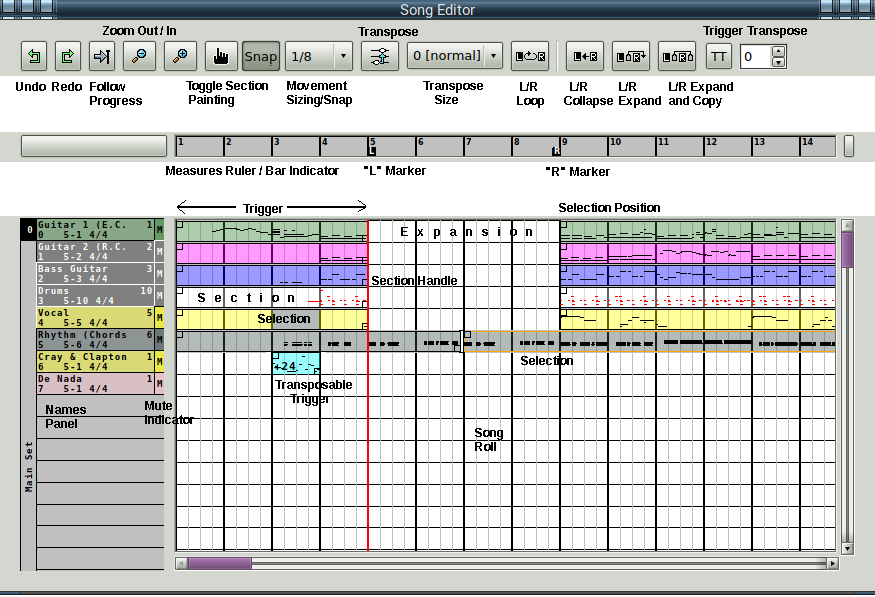
\includegraphics[scale=1.0]{song-editor/song-editor-annotated.png}
   \caption{Song Editor Window, Annotated}
   \label{fig:song_editor_window_annotated}
\end{figure}

   Note the major items shown:

   \begin{enumber}
      \item \textbf{Top Panel} (recent updates not yet shown)
      \item \textbf{Measures Ruler}
      \item \textbf{Patterns (Names) Panel}
      \item \textbf{Song Roll}
      \item \textbf{Bottom Panel}
   \end{enumber}

   The estimated duration of the tune appears at the right of the top panel.
   It is calculated from the length of patterns
   and the song triggers that may be present.
   Here are some of the features for the song editor:

   \begin{itemize}
      \item Toggling of the mute state of multiple patterns
         via the name fields of the patterns.
      \item Optional pattern coloring (selected in the Patterns panel)
      \item A configurable progress bar.
      \item \textbf{Undo} and \textbf{Redo} buttons.
      \item A \textbf{Transpose} button and transposition drop-down selector.
      \item Red coloring of events for patterns that are not transposable,
         such as drum tracks.
      \item Horizontal zoom (and a simple vertical zoom)
      via buttons and keystrokes.
      \item Opening a pattern editor via a double-click on any occupied
         track.
      \item Creating a pattern via a double-click on any unoccupied track.
   \end{itemize}

   The song editor is a bit complex; for exposition, we break it into
   sections, starting with playback keystrokes.

\subsection{Song Editor / Playback Keystrokes}
\label{subsec:song_editor_playback_keystrokes}

   The song roll (center panel)
   of the song editor provides keystrokes for starting,
   stopping, and pausing playback.
   Other keystrokes are described in
   \sectionref{subsubsec:song_editor_song_roll_keystrokes}.

%  \itempar{Stop}{song editor!stop}
%  Stops the playback of the song.
%  \index{keys!esc (stop)}
%  The keystroke for stopping playback is the \texttt{Esc} character.
%  It can be configured to be another character (such as \texttt{Space}, which
%  would make the space-bar toggle the playback status).

%  \itempar{Stop/Pause/Play}{song editor!play}
   \index{keys!space (toggle play)}
   The keystroke for starting playback is the \texttt{Space} character.
   \index{L marker}
   It starts the playback of the song at the \textbf{L marker}.
   The \textbf{L marker} serves as the start position for playback
   in the song editor.  One can change the start position only when the
   performance is not playing.
   The \texttt{Space} character also toggles playback.
   This character also rewinds the song to the beginning when stopping.

   Another keystroke for stopping playback is the \texttt{Esc} character.
   This character also rewinds the song to the beginning when stopping.
   (It also can exit paint mode, and,
   \textsl{if} the 'usr' \texttt{[pattern-editor] escape-pattern}
   option is set, will close an external song-editor window.

   \index{keys!period (pause)}
   The keystroke for pausing playback is the \texttt{Period} character.
   When used, it keep the progress at the same spot as before.

   Note that there are no stop, pause, and play buttons in the
   song editor.
   They are supplied by the main window.
   The \textbf{Song} tab can be activated in the main window to
   keep the playback buttons nearby.

\subsection{Song Editor / Top Panel}
\label{subsec:song_editor_top}

   The top panel shown earlier provides quick access to actions
   and configuration.

   \begin{enumber}
      \item \textbf{Undo}
      \item \textbf{Redo}
      \item \textbf{Follow Progress}
      \item \textbf{Zoom Out and Zoom In}
      \item \textbf{Toggle Section Painting}
      \item \textbf{Record Snap}
      \item \textbf{Grid Snap}
      \item \textbf{Transpose}
      \item \textbf{L/R Loop}
      \item \textbf{L/R Collapse}
      \item \textbf{L/R Expand}
      \item \textbf{L/R Expand and Copy}
      \item \textbf{Expand Song Roll} (not shown in figure)
      \item \textbf{Trigger Transpose}
   \end{enumber}

   \setcounter{ItemCounter}{0}      % Reset the ItemCounter for this list.

   \itempar{Undo}{song editor!undo}
   The \textbf{Undo} button rolls back the last change in the layout of a
   pattern.  Each time it is clicked, the most recent change is undone.
   Also implemented via \texttt{Ctrl-Z}.

   \itempar{Redo}{song editor!redo}
   The \textbf{Redo} button reapplies the last change undone by
   the \textbf{Undo} button.
   Also implemented via \texttt{Shift-Ctrl-Z}.

   \itempar{Zoom Out and Zoom In}{song editor!zoom}
   These buttons change the horizontal zoom.
   Zoom can also be changed via the keystrokes \texttt{z}, \texttt{0},
   and \texttt{Z}.
   Vertical zoom is also supported, by buttons to the left of the time-line and
   by keystrokes, as discussed below.

   \itempar{Follow Progress}{song editor!follow}
   \textbf{Follow Progress} toggles the mode of following progress
   for longer songs.  WHen active, the song roll pages right to keep up with
   the progress bar.

   \itempar{Toggle Section Painting}{song editor!paint}
   \textbf{Toggle Section Painting} toggles the ability
   to drag the mouse along the pattern's timeline to create triggers
   to indicate when the pattern plays.
   Short patterns will be duplicated one or more times as
   the mouse is dragged.
   This mode can alsp be changed via the keystrokes \texttt{p} and
   \texttt{x}.

   \itempar{Grid/Record Snap}{song editor!grid/record snap}
   The \textbf{Movement Sizing/Snap} setting,
   if enabled, allows not only full clips of a pattern to be added,
   but smaller intervals listed below.
   It turns on record-snap for recording live performance triggers.
   It also enables the grid snap functionality,
   which ndicates the horizontal grid snap for movement actions and trigger
   drawing.
   If disabled, it allows the trigger to be placed and to be smoothly extended
   in either direction, without snapping, when the mouse is moved left or
   right. It allows exact recording of the musician's arming/muting of
   patterns.
   Unlike the \textbf{Grid Snap} of the pattern editor, the units
   of the song editor snap value are in fractions of a measure length.
   The following values are supported:

   \textsl{1/1, 1/2, 1/4, 1/8, 1/16, and 1/32}

   Note that arming/muting can be done in the "names" panel using a
   \textsl{right-click} on the pattern name.
   Also note that changes that occur within the snap value will 
   cause odd recording, so be sure to set the snap value low enough.

   When creating triggers for patterns longer than a measure,
   the pattern may wrap, so that beginning notes appear at the end of the
   trigger, and notes can wrap around.
   To avoid this, a trick is needed:

   \begin{enumerate}
      \item Undo that trigger insertion.
      \item Select the \texttt{Length} Snap value.
      \item Insert the trigger.
      \item Click another snap value.
      \item Drag the trigger, usually to the left, until it reaches the
         desired snap location.
      \item Verify that the whole pattern is in place with the notes exactly
         placed as in the pattern.
   \end{enumerate}

   This trick is annoying, and we're not sure if note wrap-around
   is a feature or a bug.

   \itempar{Transpose}{song editor!transpose}
   \index{song transpose}
   \textbf{Transpose} consists of two controls:
   a combo-box to select the transpose direction and amount,
   and a \textbf{TT} button to reset the transposition value to 0.
   Transposition ranges from -60 to +60, or five octaves either way.
   Transpostion is applied by setting the value, and then doing
   a \texttt{Shift-left-click} on each trigger that needs that
   transposition value.

   \itempar{L/R Loop}{song editor!play loop}
   This button appears in the song editor only when it is open as
   an external window.
   This button is present in the main window, and so is not needed
   in the Song tab.
   For a description of this button, see
   \sectionref{subsubsec:introduction_loop_button}.

   \itempar{L/R Collapse}{song editor!collapse}
   This button collapses the song between the \textbf{L marker} and the
   \textbf{R marker}.
   What this means is that, if there is song material (patterns) before the
   \textbf{L marker} and after the \textbf{R marker},
   and the \textbf{Collapse} button is
   pressed, any song material between the L and R markers is erased, and
   the song material after the \textbf{R marker} is moved leftward to
   the \textbf{L marker}.
   Collapsing occurs in all tracks present in the song editor.

   \itempar{L/R Expand}{song editor!expand}
   This button expands the song between the
   \textbf{L marker} and the \textbf{R marker}.
   It inserts blank space between these markers, moving the song material
   that is after the \textbf{R marker}
   to the right by the duration of the blank space.
   Expansion occurs in all tracks present in the song editor.

   \itempar{L/R Expand and Copy}{song editor!expand and copy}
   This button expands the song between the \textbf{L marker} and the
   \textbf{R marker} much like the \textbf{Expand} button.
   However, it also copies the original data that is present after the
   \textbf{R marker}, and pastes it into the newly-available space between
   the L and R markers.

   \itempar{Expand Song Roll}{song editor!expand song roll}
   Sometimes one might come to the end of the song and still want to
   add more triggers.
   Clicking this button expands the song roll to the right, adding
   more room for triggers.

   \itempar{Trigger Transpose}{song editor!trigger transpose}
   This button and spin-box support making trigger selections or segments
   transposable during play-back.  This feature is very useful
   for patterns that repeat many times, but are shifted in pitch at various
   points.
   The transposition value ranges from -60 to 0 to +60, in units of semitones.
   The button resets the value to 0.
   To apply a transposition value, first set it in the spin-box.
   Then carefully \textsl{shift-left-click}
   on the desired segment(s) to transpose.
   A number with a plus-or-minus will appear at the left of the segment to
   indicate a non-zero transposition.
   The transposition value will be saved with the trigger when the song is
   saved.

\subsection{Song Editor / Measures Ruler}
\label{subsec:song_editor_measures_ruler}

   \index{measures ruler}
   The measures ruler ("bar indicator", or "Time")
   consists of a \textsl{timeline} at the top and the 
   \textbf{L marker} and \textbf{R marker} mentioned above.
   The \textsl{measures ruler} is the ruled and numbered section at the top
   of the arrangement panel.  It provides a place to put the left and right
   markers.  In the \textsl{Seq24} documentation, it is called the "bar
   indicator".
   There are some hidden details (tricks) in the measures panel.

   \begin{itemize}
      \item \textbf{In the upper half} of the time-line,
         the mouse pointer changes to a vertical pointer.
         Clicking there then shows a red dot; these mark
         the starting position of playback.
         This is useful for review.
      \item \textbf{In the lower half} of the time-line,
         the mouse pointer changes to a "finger" icon.
         \textsl{Left-clicking} there then moves the \textbf{L}
         marker to that point.
         \textsl{Right-clicking} there moves the \textbf{R} marker to that point.
         (\textbf{R} will never precede \textbf{L}, though).
         If the \textbf{Loop} button in the main window is active, then
         playback will loop between the \textbf{L} and \textbf{R} buttons.
         This looping now works with both Live and Song modes.
   \end{itemize}

   \index{measures ruler!left-click}
   \textsl{Left-click} in the bottom-half of the
   measures ruler to move and drop an
   \index{L anchor}
   \index{L marker}
   \textbf{L marker} (\textbf{L anchor}) on the measures ruler.
   \index{measures ruler!right-click}
   \textsl{Right-click} in the bottom-half of the measures ruler to drop an
   \index{R anchor}
   \index{R marker}
   \textbf{L marker} (\textbf{R anchor}) on the measures ruler.
   
   These markers denote the time interval from the left of the 
   \textbf{L} marker to the right of the \textbf{R} marker.
   Once these markers are in place, one can then use
   the \textsl{Collapse} and \textsl{Expand} buttons to modify the
   placement of the pattern events.
   Note that the \textbf{L marker} serves as the start position for playback
   in the song editor even when not looping.
   One can change the start position only when the
   performance is not playing.

   \index{marker!mode}
   \index{marker!movement}
   Another way to move the \textbf{L} and \textbf{R} markers has been added.
   To select which marker will move, click the upper half of the time
   strip (otherwise, the \textbf{L} will move,
   prematurely) to give it keyboard focus.
   Then press the lower-case
   \index{keys!l}
   \texttt{l} key or the lower-case
   \index{keys!r}
   \texttt{r} key.
   \textsl{There is no visual feedback that one is in the movement mode.}
   Then press the \texttt{Left-Arrow} or \texttt{Right-Arrow}
   key to move the selected marker.
   Also included at the same level as the measures ruler are the buttons
   \textbf{-}, \textbf{0}, and \textbf{+},
   which are used for vertical zoom, as described below.

\subsection{Song Editor / Patterns (Names) Panel}
\label{subsec:song_editor_patterns_panel}

   The patterns panel is at the left of the song roll.
   Here are the items to note in the pattern-names panel:

   \begin{enumber}
      \item \textbf{Number}.
         The number of the screen set.
      \item \textbf{Title}.
         \index{pattern!title}
         \index{pattern!name}
         The title is the name of the pattern, for easy reference.
      \item \textbf{Color}.
         If a color is provided for the pattern, then that color is shown.
         Also, as an editing aid, the pattern over which the mouse is hovering
         is shown in a brighter version of the color.
      \item \textbf{Channel}.
         \index{pattern!channel}
         The channel number appears (redundantly)
         at the right of the title.
      \item \textbf{Buss-Channel}.
         \index{pattern!buss-channel}
         This pair of numbers shows the MIDI buss number used in the pattern
         and the channel used for the pattern.
      \item \textbf{Beat/Measure}.
         \index{pattern!beat}
         This pair of numbers is the standard time-signature of the pattern.
      \item \textbf{Trigger Count}.
         \index{pattern!trigger count}
         This number shows the number of triggers present in the pattern.
      \item \textbf{Mute Indicator}.
         \index{song editor!mute indicator}
         The letter \textbf{M} is in a grey box if the track/pattern
         is muted via song playback,
         and a white (or colored) box if it is unmuted in song playback.
         \textsl{Left-clicking} on the \textbf{M} (or the name of the pattern)
         mutes/unmutes the pattern.
         \index{left click}
         Song muting is effected via a \textsl{left-click} on the pattern name.
         This is also useful in song-recording (where the triggers are recorded).
         \index{shift left click}
         If the Shift key is held while \textsl{left-clicking}
         on the M or the pattern name, then
         the mute/unmute state of every other active pattern is toggled.
         This feature is useful for isolating a single track or pattern.
         \index{right click}
         Normally, one records song triggers using the grid buttons or MIDI
         control to turn patterns on and off.
         One can also \textsl{right-click} on the pattern
         name during song-record and
         thereby see the trigger(s) being created.
      \item \textbf{Empty Track}.
         Completely empty tracks (no track events or meta events)
         are indicated by a dark-gray filling in the pattern column.
         Tracks that have only meta information, but no playable event, are
         indicated by a yellow filling in the pattern column.
   \end{enumber}

   The patterns column shows a list of all of the patterns that have been
   created in the current song.  Each pattern in this list has a track of
   pattern layouts associated with it in the piano roll section.

   \index{patterns column!left-click}
   \index{patterns column!ctrl-left-click}
   \index{song editor!muting}
   \textsl{Left-clicking} on the pattern name or the \textbf{M} toggles the muting
   (arming) status of the track.
   It does the same thing if the \texttt{Ctrl} key is held at the same time.

   \index{pattern!shift-left-click}
   \index{song editor!inverse muting}
   \index{song editor!solo}
   \index{shift-left-click solo}
   \textsl{Shift-left-clicking} on the pattern name
   or the \textbf{M} button toggles the muting
   (arming) status of \textsl{all other tracks} except the track that was
   selected.  This action is useful for quickly listening to a single sequence
   in isoloation.

   \index{patterns column!double-click}
   \textsl{Double-clicking} on the pattern name
   will either create a new pattern or open up the corresponding pattern
   window.
   This feature saves having to move to the live grid.

% Think about implementing this feature for real. At least partially.
%
%  \index{patterns column!right-click}
%  \textsl{Right-clicking} on the pattern name or
%  the \textbf{M} button brings up the same
%  pattern editing menu as discussed in
%  \sectionref{subsubsec:patterns_pattern_filled}.
%  Recall that this context menu has the following entries:
%  \textbf{Edit...}, \textbf{Event Edit...}, \textbf{Cut}, \textbf{Copy},
%  \textbf{Song}, \textbf{Disable Transpose}, and \textbf{MIDI Bus}.

\subsection{Song Editor / Song Roll}
\label{subsec:song_editor_song_roll}

   The "Song Roll" section of the arrangement panel is where patterns or
   subsections are inserted, deleted, shrunk, lengthened, or moved.
   Actions can be done via the mouse or keyboard.

\subsubsection{Song Editor / Song Roll / Layout}
\label{subsubsec:song_editor_song_roll_layout}

   The song/piano roll provides one line (track) per pattern.
   It provides another way (besides the live grid) to control
   and lay out patterns.
   Patterns can be set up with multiple triggers and can be
   brought up for editing.
   Here are features to note in the annotated piano roll area:

   \begin{enumber}
      \item \textbf{Note Events}.
         \index{song editor!note events}
         Note in the pattern are shown as thin horizontal lines.
         They can be edited in the pattern editor's piano roll,
         and in the event editor.
      \item \textbf{Tempo Events}.
         \index{song editor!tempo events}
         Tempo events in the pattern are shown as very small squares.
         They can be edited in the pattern editor's data panel,
         and in the event editor.
      \item \textbf{Pattern Access}. (Since version 0.99.10).
         Double-clicking (if enabled in the 'rc' file) on a track
         representing an existing pattern will bring up an external
         pattern editor windows.
         Double-clicking on an empty track will create a new pattern
         and bring up its pattern editor.
         This new functionality is merely for convenience.
      \item \textbf{Trigger Creation}.
         By click-dragging the mouse on a track, in paint mode,
         a series of triggers can be
         created; they indicate where the track will be unmuted and playing.
         See below for more information about triggers.
      \item \textbf{Selection}.
         Clicking inside a trigger selects it.
         Selection is denoted by an orange rectangle around the trigger
         and a dark grey color in the trigger.
         A pattern subsection can be moved by the mouse and deleted by
         keystrokes.
      \item \textbf{De-selection}.
         \index{song editor!section deselection}
         \textsl{Left-clicking} or \textsl{right-clicking} in
         an empty area of the song roll
         will deselect the selection.
      \item \textbf{Selection Movement}.
         \index{song editor!selection movement}
         If one grabs (\textsl{left-click}) inside
         the pattern or pattern subsection, that item can be moved
         horizontally, as long as there is room.
      \item \textbf{Section Length ("handle")}.
         \index{song editor!handle}
         \index{song editor!section length}
         The small squares in two corners of the patterns are the section
         "handles".
         By grabbing a handle with a \textsl{left-click},
         the handle can be moved
         horizontally to either lengthen or shorten the pattern to the nearest
         snap position, if there is room to move in the desired direction.
      \item \textbf{Pattern Subsectioning}.
         \index{song editor!split pattern}
         \index{song editor!middle click}
         \index{pattern subsection}
         A \textsl{middle-click} (or \textsl{ctrl-left-click})
         inside a pattern inserts a selection position
         marker in it, breaking the pattern into two equal pieces.
         We call each piece a \textsl{pattern subsection}.
         This division can be done over and over.
         There are also options for splitting at the nearest snap point.
      \item \textbf{Expansion}.
         \index{song editor!section expansion}
         Originally, all the long patterns of this sample song were continuous.
         But, by setting the L and R markers, and using the \textbf{Expand}
         button, we opened up some silent space in the song, just to be able
         to show it off.
   \end{enumber}

   The \textsl{Seq24} help files refer to work in the song editor as the
   "Performance Editor" or "Performance Mode".  Adding a pattern in this
   window is a bit like adding a note in the pattern editor.
   One clicks, holds, and drags the mouse to insert a copy or copies of the
   pattern associated with the row in which one is dragging.
   The longer one drags, the more copies of the pattern that are inserted.

   \index{song editor!right-click-hold}
   \index{song editor!draw}
   \index{paint mode}
   \textsl{Right-click} on the arrangement panel (roll) to enter
   paint mode, and hold the button.
   Paint mode does not work while the sequence is playing.
   Another way to turn on painting is to
   make sure that the performance editor piano roll has the
   keyboard focus by \textsl{left-clicking} in it, then press the
   \texttt{p} or \texttt{i} key to enter the paint/insert mode, and
   \texttt{x} (or \texttt{Esc} if not playing) to escape it.
   See \sectionref{subsubsec:song_editor_song_roll_keystrokes}.

   \index{zoom}
   \index{song editor!horizontal zoom}
   The song editor supports horizontal zoom in the piano roll.
   This feature is accessible via the "magnifying glass" buttons, and also
   accessible via the keystrokes \textbf{z}, \textbf{0}, and \textbf{Z}.
   The zoom feature also modifies the time-line.

   \index{zoom}
   \index{song editor!vertical zoom}
   The song editor supports limited vertical zoom in the piano roll.
   This feature is accessible via the \textbf{-}, \textbf{0}, and
   \textbf{+} buttons, and also
   accessible via the keystrokes \textbf{v}, \textbf{0}, and \textbf{V}.

   \index{song editor!left-click-right-hold}
   \index{song editor!insert}
   A \textsl{left-click} with a simultaneous
   \textsl{right-click-hold} inserts one copy of the
   pattern.  The inserted pattern shows up as a box with a tiny
   representation of the notes visible inside.  Some patterns can
   be less than a measure in length, resulting in a tiny box.
   \index{song editor!right-left-hold-drag}
   \index{song editor!multiple insert}
   To keep adding more copies of the pattern, continue to hold both buttons
   and drag the mouse rightward.

   \index{song editor!middle-click}
   \textsl{Middle-click} (or \textsl{ctrl-left-click})
   on a trigger in a pattern row
   to splits the trigger into two triggers.
   \index{pattern!split}
   \index{song editor!pattern subsection}
   This splits the pattern into two equal \textsl{pattern subsections}.
   Each \textsl{middle-click} on the pattern adds a new selection position,
   halving the size of the subsections as more pattern subsections are
   added.  The \texttt{allow\_snap\_split} option in the 'rc' file
   allows the split to be made at the nearest snap point instead of in the
   middle.

   \index{song editor!left-click}
   \index{song editor!selection}
   When a pattern or a pattern subsection is
   \textsl{left-clicked} in the piano
   roll, it is marked with a dark gray filling.
   It can then be moved horizontally if there is room, or be deleted or copied
   for later pasting.

   \index{song editor!right left click}
   \index{song editor!deletion}
   When a 
   \textsl{right-left-click} action is done in this gray area, the result
   is to \textsl{delete} that pattern section or subsection.
   \index{keys!delete}
   One can also hit the \texttt{Delete} key.

   \index{song editor!double-click}
   \textsl{Double-click} on one of the trigger bars
   will either create a new pattern or open up the corresponding pattern
   window.
   This feature saves having to move to the live grid.

\subsubsection{Song Editor / Song Roll / Keystrokes}
\label{subsubsec:song_editor_song_roll_keystrokes}

   There are a number of useful keystrokes in the song roll that can be used
   once is has focus, by clicking in it.

   \begin{itemize}
      \item Enter "paint" mode.
         The \texttt{p} key enters paint mode, where additional triggers
         can be added by click-dragging on a pattern row.
         The \texttt{x} key leaves this mode.
         The "finger" button and the mouse cursor both indicate the status.
      \item Start/Pause button functionality.
         When the song roll has keyboard focus,
         the \texttt{Space} key starts and stops playback, rewinding to the
         beginning when stopped.
         The \texttt{.} (period) key starts and pauses playback, without
         rewinding.
         This functionality is similar to that of the main window, but
         these keys are not reconfigurable in the song roll.
      \item Undo / Redo / Cut / Copy / Paste of a selected section.
         Provided by buttons and by these keystrokes:
         \begin{itemize}
            \item \texttt{Ctrl-Z}. Undo.
            \item \texttt{Shift-Ctrl-Z}. Redo.
            \item \texttt{Ctrl-X}. Cut.  Removes the selection.
            \index{keys!backspace}
            \index{keys!delete}
            \index{keys!ctrl-x}
            Can also be done with the \texttt{Delete} and
            \texttt{Backspace} keys.
            The deletion can be undone.
            \item \texttt{Ctrl-C}. Copy.
         \index{keys!ctrl-c}
         \index{keys!copy}
            Copies the trigger for later usage.
            \item \texttt{Ctrl-V}. Paste.
            \index{keys!ctrl-v}
            \index{keys!paste}
            Puts the roll into paste mode.
            When inserted, each insert goes immediately
            after the current item or the previous insertion.  The same can be
            done for whole patterns.
         \end{itemize}
      \item Horizontal (Time) Zoom.  These keystrokes work similarly to the
      pattern editor's piano roll.
         Provided by buttons and by these keystrokes:
         \index{keys!shift-z}
         \texttt{Z}. Zoom in horizontally (i.e. in time).
         \index{keys!z}
         \texttt{z}. Zoom out horizontally.
         \index{keys!0}
         \texttt{0}. Reset zoom both horizontally and vertically.
      \item Vertical (Time) Zoom.  These keystrokes work similarly to the
         pattern editor's piano roll.
         However, there are only three levels of
         vertical zoom:  half-size, normal, and double-size.
         \index{keys!shift-V}
         \texttt{V}. Zoom in vertically to get a better view of the patterns
            and a large grab handle.
         \index{keys!v}
         \texttt{v}. Zoom out vertically to see more tracks.
         \texttt{0}. Reset zoom both horizontally and vertically.
      \item Scrolling.
         \index{keys!arrows}
         The arrow keys will move the piano row up, down, left, and right.
         \index{keys!hjkl}
         In addition, the "vi" keys \texttt{h}, \texttt{j}, \texttt{k}, and
         \texttt{l} will act like the arrow keys.
         The mouse scroll wheel can also be used to move the panes around.
         For implementation reasons, the scroll wheel is active
         \textsl{only} in the piano roll.
      \item Paging.
         One can page up and down vertically in the arrangement
         panel using the
         \index{keys!page-up}
         \texttt{Page Up} and 
         \index{keys!page-down}
         \texttt{Page Down} keys.
         One can page left and right horizontally in the arrangement
         panel using the
         \index{keys!up-arrow} \texttt{Up-Arrow} and 
         \index{keys!down-arrow} \texttt{Down-Arrow} keys.
   \end{itemize}

\subsection{Song Editor / Bottom Panel}
\label{subsec:song_editor_bottom}

   The bottom panel is simple, consisting of a stock horizontal scroll bar.

\begin{comment}

   ...and a small button, called the \textbf{Grow} button, labelled with a
   "\textbf{$>$}".
   \index{grow button}
   \index{song editor!grow}
   The \textbf{Grow} button adds to the number of measures that exist
   in the song editor. The visual effect is very subtle, resulting only
   in a small change in the thumb of the horizontal scroll-bar, unless one
   is at the right end of the piano roll.  Then, one can see the added
   measures.  Usually about 128 at a time are added, but this depends on the
   value of PPQN in force.

\end{comment}

%-------------------------------------------------------------------------------
% vim: ts=3 sw=3 et ft=tex
%-------------------------------------------------------------------------------
